\begin{problem}%
{Фи от Эн}%
{\textsl{стандартный ввод}}%
{\textsl{стандартный вывод}}%
{1 секунда}%
{64 мегабайта}{}

\begin{center}
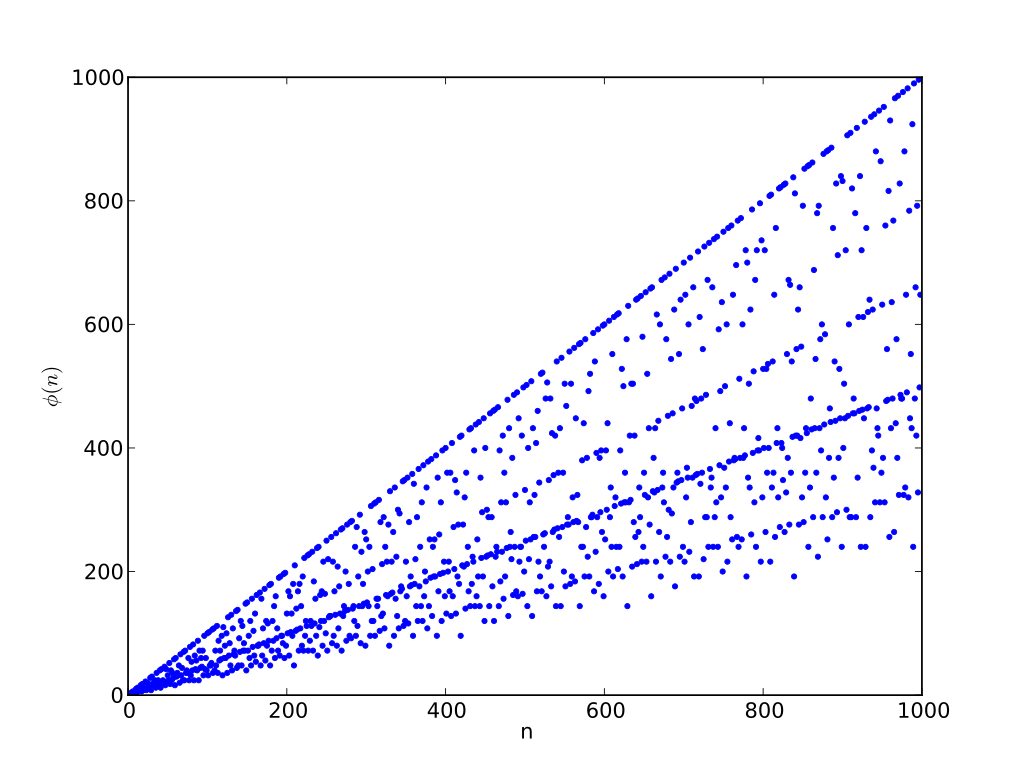
\includegraphics[scale=0.5]{images/EulerPhi.png}
\end{center}

\InputFile

В единственной строке вводится целое число $x$ ($1 \le x \le 10^5$).

\OutputFile

Выведите одно целое число.

\Examples

\begin{example}
\exmp{
1
}{%
1
}%
\exmp{
2
}{%
1
}%
\end{example}
\end{problem}
